%%%%%%%%%%%%%%%%%%%%%%%%%%%%%%%%%%%%%%%
% Wenneker Resume/CV
% LaTeX Template
% Version 1.1 (19/6/2016)
%
% This template has been downloaded from:
% http://www.LaTeXTemplates.com
%
% Original author:
% Frits Wenneker (http://www.howtotex.com) with extensive modifications by 
% Vel (vel@LaTeXTemplates.com)
%
% License:
% CC BY-NC-SA 3.0 (http://creativecommons.org/licenses/by-nc-sa/3.0/
%
%%%%%%%%%%%%%%%%%%%%%%%%%%%%%%%%%%%%%%

%----------------------------------------------------------------------------------------
%	PACKAGES AND OTHER DOCUMENT CONFIGURATIONS
%----------------------------------------------------------------------------------------

\documentclass[a4paper,12pt]{memoir} % Font and paper size
\usepackage[dvips]{graphicx}
\graphicspath{{noiseimages/}}
\usepackage[T1,T2A]{fontenc}
\usepackage[utf8x]{inputenc}
\usepackage[english,russian]{babel}
%%%%%%%%%%%%%%%%%%%%%%%%%%%%%%%%%%%%%%%%%
% Wenneker Resume/CV
% Structure Specification File
% Version 1.1 (19/6/2016)
%
% This file has been downloaded from:
% http://www.LaTeXTemplates.com
%
% Original author:
% Frits Wenneker (http://www.howtotex.com) with extensive modifications by 
% Vel (vel@latextemplates.com)
%
% License:
% CC BY-NC-SA 3.0 (http://creativecommons.org/licenses/by-nc-sa/3.0/)
%
%%%%%%%%%%%%%%%%%%%%%%%%%%%%%%%%%%%%%%%%%

%----------------------------------------------------------------------------------------
%	PACKAGES AND OTHER DOCUMENT CONFIGURATIONS
%----------------------------------------------------------------------------------------

\usepackage{XCharter} % Use the Bitstream Charter font
\usepackage[utf8]{inputenc} % Required for inputting international characters
\usepackage[T1]{fontenc} % Output font encoding for international characters

\usepackage[top=1cm,left=1cm,right=1cm,bottom=1cm]{geometry} % Modify margins

\usepackage{graphicx} % Required for figures

\usepackage{flowfram} % Required for the multi-column layout

\usepackage{url} % URLs

\usepackage[usenames,dvipsnames]{xcolor} % Required for custom colours

\usepackage{tikz} % Required for the horizontal rule

\usepackage{enumitem} % Required for modifying lists
\setlist{noitemsep,nolistsep} % Remove spacing within and around lists

\setlength{\columnsep}{\baselineskip} % Set the spacing between columns

% Define the left frame (sidebar)
\newflowframe{0.2\textwidth}{\textheight}{0pt}{0pt}[left]
\newlength{\LeftMainSep}
\setlength{\LeftMainSep}{0.2\textwidth}
\addtolength{\LeftMainSep}{1\columnsep}
 
% Small static frame for the vertical line
\newstaticframe{1.5pt}{\textheight}{\LeftMainSep}{0pt}
 
% Content of the static frame with the vertical line
\begin{staticcontents}{1}
\hfill
\tikz{\draw[loosely dotted,color=RoyalBlue,line width=1.5pt,yshift=0](0,0) -- (0,\textheight);}
\hfill\mbox{}
\end{staticcontents}
 
% Define the right frame (main body)
\addtolength{\LeftMainSep}{1.5pt}
\addtolength{\LeftMainSep}{1\columnsep}
\newflowframe{0.7\textwidth}{\textheight}{\LeftMainSep}{0pt}[main01]

\pagestyle{empty} % Disable all page numbering

\setlength{\parindent}{0pt} % Stop paragraph indentation

%----------------------------------------------------------------------------------------
%	NEW COMMANDS
%----------------------------------------------------------------------------------------

\newcommand{\userinformation}[1]{\renewcommand{\userinformation}{#1}} % Define a new command for the CV user's information that goes into the left column

\newcommand{\cvheading}[1]{{\Huge\bfseries\color{RoyalBlue} #1} \par\vspace{.6\baselineskip}} % New command for the CV heading
\newcommand{\cvsubheading}[1]{{\Large\bfseries #1} \bigbreak} % New command for the CV subheading

\newcommand{\Sep}{\vspace{1em}} % New command for the spacing between headings
\newcommand{\SmallSep}{\vspace{0.5em}} % New command for the spacing within headings

\newcommand{\aboutme}[2]{ % New command for the about me section
\textbf{\color{RoyalBlue} #1}~~#2\par\Sep
}
	
\newcommand{\CVSection}[1]{ % New command for the headings within sections
{\Large\textbf{#1}}\par
\SmallSep % Used for spacing
}

\newcommand{\CVItem}[2]{ % New command for the item descriptions
\textbf{\color{RoyalBlue} #1}\par
#2
\SmallSep % Used for spacing
}

\newcommand{\bluebullet}{\textcolor{RoyalBlue}{$\circ$}~~} % New command for the blue bullets
 % Include the file specifying document layout and packages

%----------------------------------------------------------------------------------------
%	NAME AND CONTACT INFORMATION 
%----------------------------------------------------------------------------------------

\userinformation{ % Set the content that goes into the sidebar of each page
\begin{flushright}
% Comment out this figure block if you don't want a photo
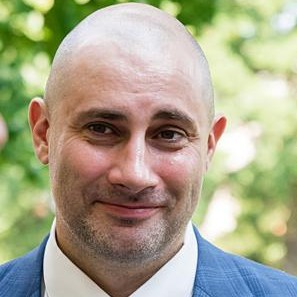
\includegraphics[width=0.6\columnwidth]{photo.jpg}\\[\baselineskip] % Your photo
\small % Smaller font size
	\begin{otherlanguage*}{russian}
Сергей Рязанов \\ % Your name
	\end{otherlanguage*}
\url{majo78@mail.ru} \\ % Your email address
\url{www.majotrade.net} \\ % Your URL
+7 (911) 934-46-49 \\ % Your phone number
\Sep % Some whitespace
\textbf{Адрес:} \\
Хазова 10-108 \\ % Address 1
Санкт-Петербург, Пушкин 196605 \\ % Address 2
Россия \\ % Address 3
\vfill % Whitespace under this block to push it up under the photo
\end{flushright}
}

%----------------------------------------------------------------------------------------

\begin{document}

\userinformation % Print your information in the left column

\framebreak % End of the first column

%----------------------------------------------------------------------------------------
%	HEADING
%----------------------------------------------------------------------------------------

\cvheading{Сергей Рязанов} % Large heading - your name

\cvsubheading{C++ Разработчик} % Subheading - your occupation/specialization

%----------------------------------------------------------------------------------------
%	ABOUT ME
%----------------------------------------------------------------------------------------

\aboutme{Обо мне}{С 2006 года работаю на финансовых рынках. ММВБ, ФОРТС, NYSE, Binance.
В 2009-2011гг. работал трейдером в брокерской компании. В настоящий момент являюсь частным
трейдером на криптовалютном рынке и управляющим крипто-активами в инвестиционном фонде.
Несколько лет работал копирайтером и SEO-аналитиком. Умею создавать веб-сайты на wordpress.
Несколько лет создавал торговых роботов в программе TsLab. Сейчас разрабатываю собственное
ПО для Linux на C++}

%----------------------------------------------------------------------------------------
%	EDUCATION
%----------------------------------------------------------------------------------------

\CVSection{Образование}

%------------------------------------------------

\CVItem{https://www.sololearn.com/profile/13138948}{sololearn.com}
\begin{figure}[h]
\begin{minipage}[h]{0.49\linewidth}
\center{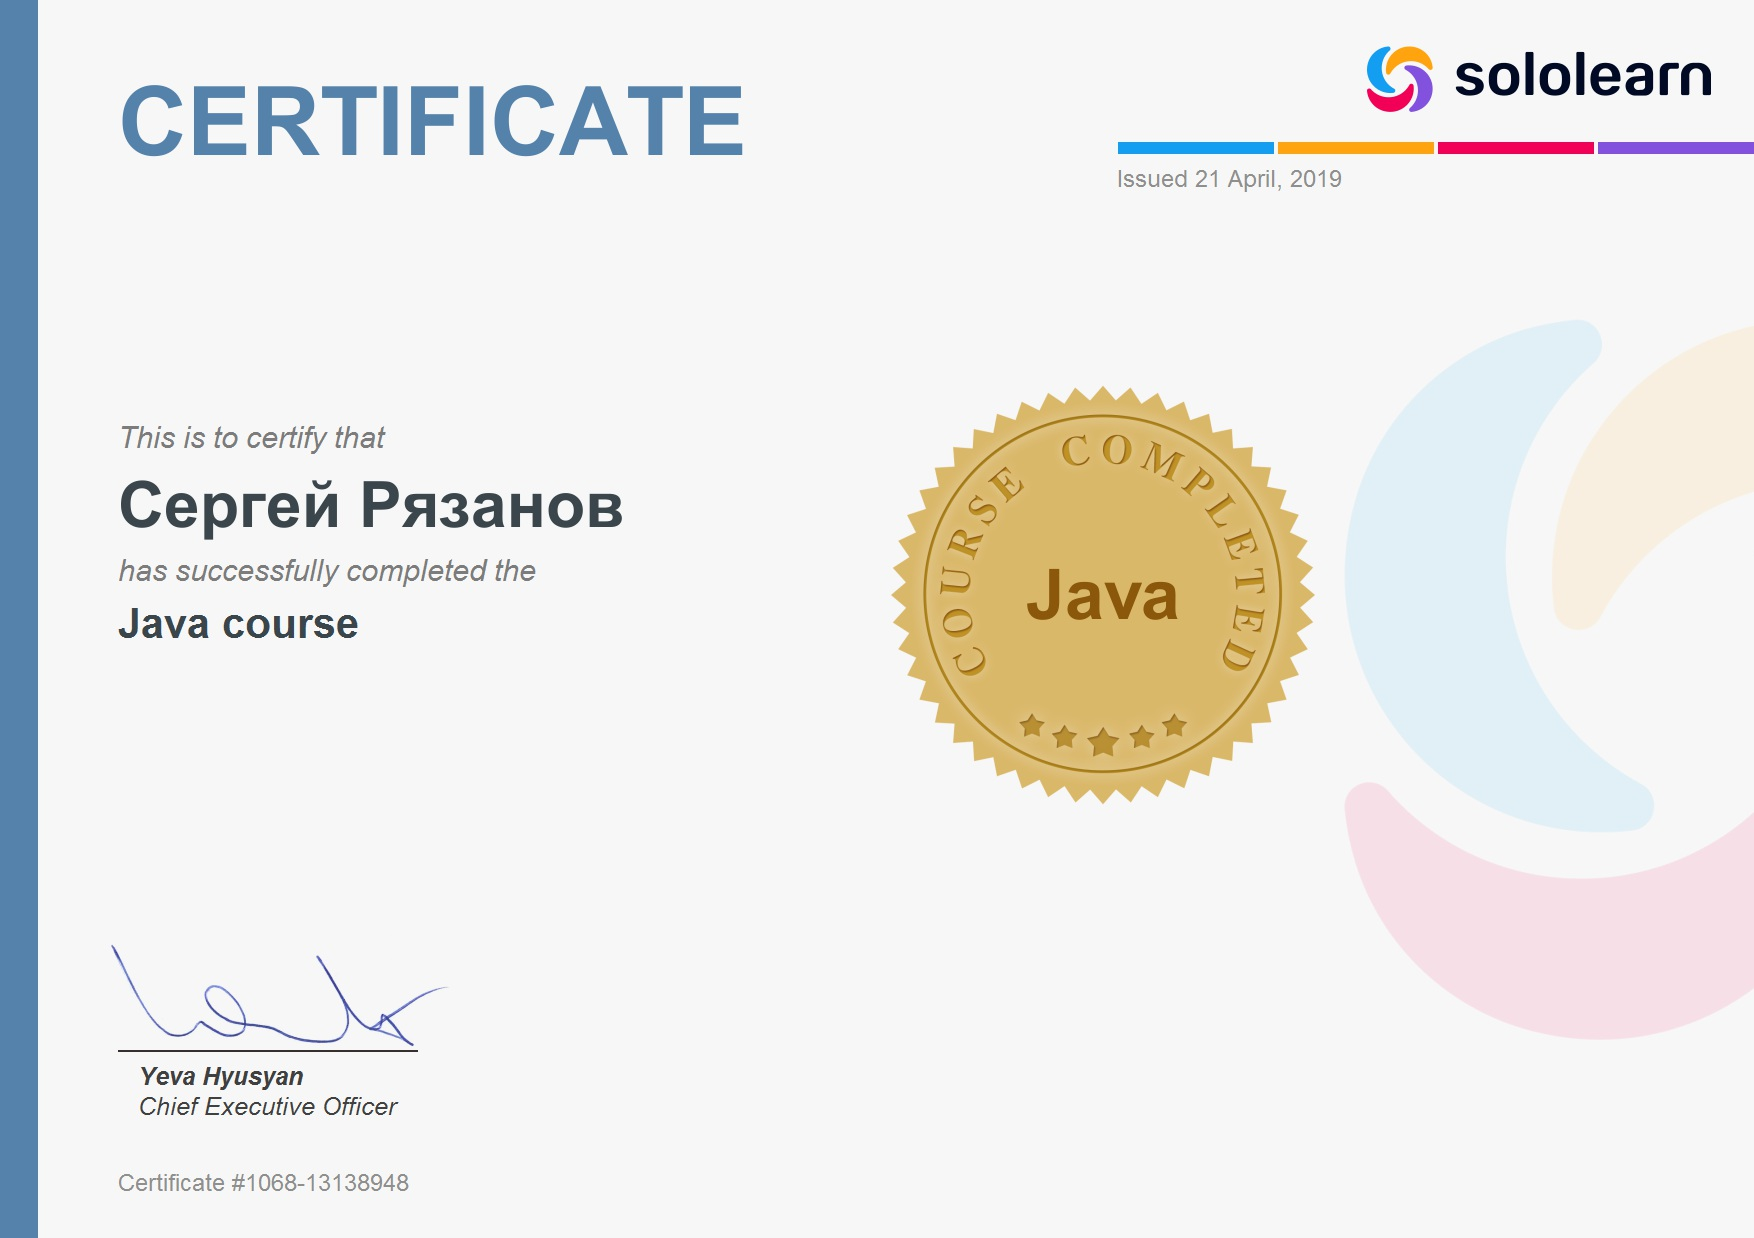
\includegraphics[width=0.5\linewidth]{java} \\ }
\end{minipage}
\hfill
\begin{minipage}[h]{0.49\linewidth}
\center{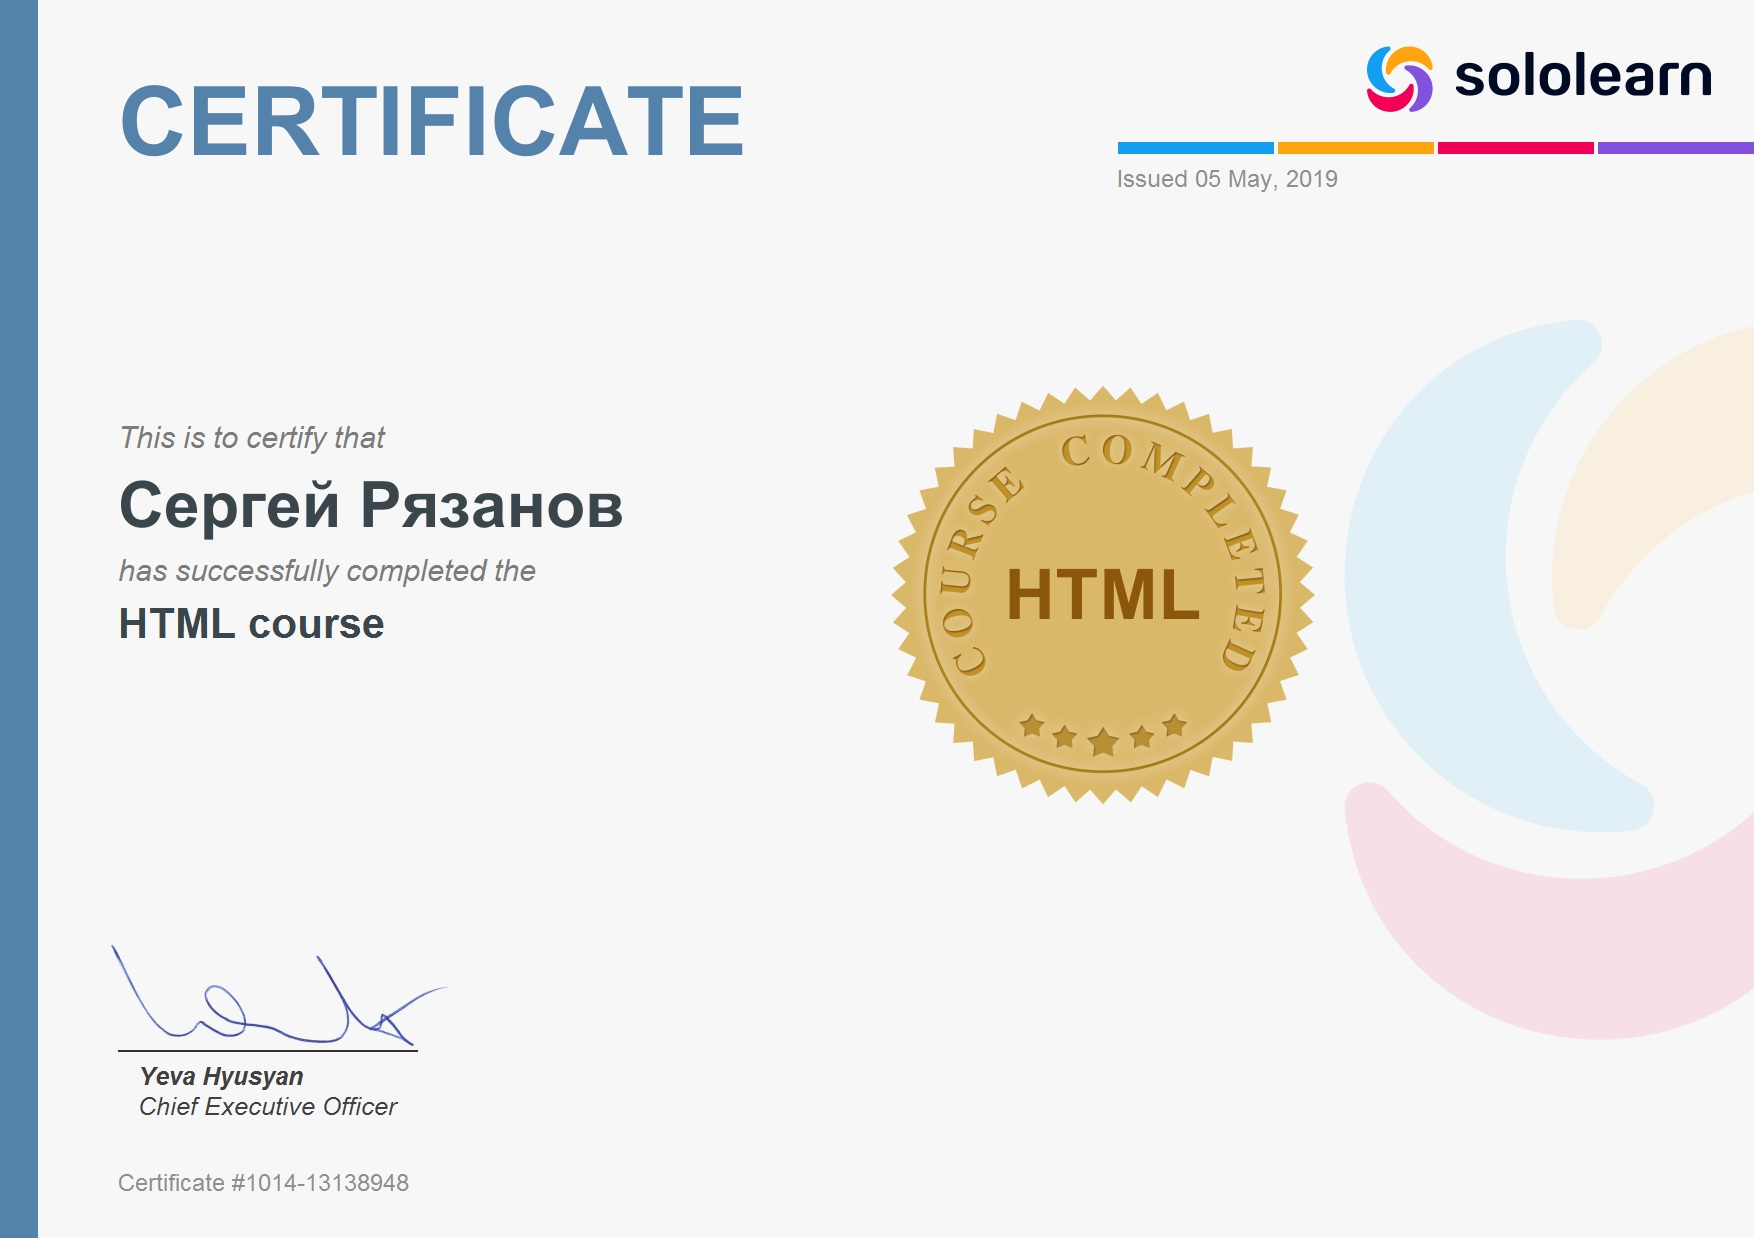
\includegraphics[width=0.5\linewidth]{html} \\ }
\end{minipage}
\end{figure}
%------------------------------------------------

\CVItem{https://go.skillbox.ru/profession/paket-c-plus-plus}{2021-2022 skillbox.ru}

%------------------------------------------------

\CVItem{https://github.com/MajotraderLuky}{GitHub}

%------------------------------------------------

\Sep % Extra whitespace after the end of a major section

%----------------------------------------------------------------------------------------
%	EXPERIENCE
%----------------------------------------------------------------------------------------

\CVSection{Опыт}

%------------------------------------------------

\CVItem{2009-2011 \textit{трейдер} ЗАО "Конто"}{
Обязанности:
\begin{itemize}
	\item Управление сервером Quik
	\item Управление счетами клиентов \textsc{трейдер}:
	\begin{itemize}
		\item ММВБ
		\item ФОРТС:
		\begin{itemize}
			\item торговля акциями и фьючерсами;
			\item торговля опционами.
		\end{itemize}
\end{itemize}
}

%------------------------------------------------

\CVItem{2011 - 2014, \textit{Копирайтер и SEO-аналитик}, Freelance}{Наполнение вебсайтов контентом - поднятие их в поисковой выдаче.}

%------------------------------------------------

		\CVItem{2014-2021, \textit{Трейдер в инвестиционной компании}, Freelance}{Управление средствами клиентов на криптовалютной бирже.}

\Sep % Extra whitespace after the end of a major section

%----------------------------------------------------------------------------------------
%	COMMUNICATION SKILLS
%----------------------------------------------------------------------------------------

\Sep % Extra whitespace after the end of a major section

%----------------------------------------------------------------------------------------
%	SKILLS
%----------------------------------------------------------------------------------------

\CVSection{Software Development Skills}

%------------------------------------------------

\CVItem{Программирование}
{\begin{tabular}{p{0.2\textwidth} p{0.2\textwidth} p{0.2\textwidth}}
\bluebullet Java &  \bluebullet Bash & \bluebullet Python\\
\bluebullet C++ &  \bluebullet Html & \bluebullet CSS\\
\end{tabular}}

%------------------------------------------------

\CVItem{OS}
{\begin{tabular}{p{0.2\textwidth} p{0.2\textwidth} p{0.2\textwidth}}
 \bluebullet Linux &  \bluebullet Windows & \bluebullet Android\\
\end{tabular}}

%------------------------------------------------

\Sep % Extra whitespace after the end of a major section

%----------------------------------------------------------------------------------------
%	NEW PAGE DELIMITER
%	Place this block wherever you would like the content of your CV to go onto the next page
%----------------------------------------------------------------------------------------

\clearpage % Start a new page
\begin{table}[h]
  \centering
  \begin{tabular}{p{4cm}cp{0cm}}
   \userinformation
  \end{tabular}
\end{table}
%\userinformation % Print your information in the left column
\framebreak % End of the first column

%----------------------------------------------------------------------------------------
%	AWARDS
%----------------------------------------------------------------------------------------

%\CVSection{Awards}

%------------------------------------------------

%\CVItem{2010, \textit{Postgraduate Scholarship}, Cornell University}{Awarded to the top student in their final year of a Bachelors degree.}

%------------------------------------------------

\Sep % Extra whitespace after the end of a major section

%----------------------------------------------------------------------------------------
%	INTERESTS
%----------------------------------------------------------------------------------------

\CVSection{Интересы}

%------------------------------------------------

\CVItem{Профессиональные}{C++, написание ПО для Linux, глубокое понимание языка программирования, алгоритмическая торговля, инвестиции.}

%------------------------------------------------

\CVItem{Личные}{Книги, кино, спорт, путешествия, овощеводство на даче.}

%------------------------------------------------
\CVSection{Какую работу я ищу}

\CVItem{Мои пожелания}{Ищу работу связанную с программированием на C++, мне бы хотелось изучить этот мощный язык и ежедневно писать код на нём. Изучать документацию. Мне бы хотелось стать участником интересного проекта и приносить пользу коллегам. Каждый день хотел бы узнавать что-то новое о C++ и решать всё более сложные задачи. На такую работу я буду ходить с удовольствием, и это залог моего личного успеха и гарантия быстрого вовлечения в рабочий процесс.}

\Sep % Extra whitespace after the end of a major section

%----------------------------------------------------------------------------------------

\end{document}
